\documentclass[11pt,a4paper]{article}

\usepackage[margin=2.2cm]{geometry}
\usepackage{amsmath,amssymb,bm}
\usepackage[T1]{fontenc}
\usepackage[utf8]{inputenc}
\usepackage{natbib}
\usepackage{booktabs}
\usepackage{graphicx}
\usepackage{hyperref}
\hypersetup{colorlinks=true,linkcolor=blue!50!black,citecolor=blue!50!black,urlcolor=blue!50!black}
\usepackage{xcolor}
\usepackage{float}

\bibliographystyle{plainnat}
\setcitestyle{authoryear,round}
\sloppy

\newcommand{\pMpc}{\,{\rm pMpc}}
\newcommand{\Msun}{\,M_\odot}
\newcommand{\Kini}{K_{\rm ini}}

\title{\bf Cosmic-Ray Electrons, the Str\"omgren Radius, and Patchy Reionization:\\
Response to \texttt{master\_plan}\\[2mm]
\large Response record for \texttt{Master\_Plan\_Ionization\_power/}, following Master Rule 2}
\author{Prepared for L.\ Carvalho}
\date{6 September 2026}

\begin{document}
\maketitle

\begin{abstract}
\noindent
\texttt{Paper\_1/master\_plan} asks whether cosmic-ray (CR) electrons injected by an early
star-forming galaxy can significantly modify that galaxy's own Str\"omgren/H\,\textsc{ii}-bubble
evolution, and what that implies for the patchy-reionization history. This note (1) identifies
five physical plot holes/inconsistencies in the proposed reasoning chain, (2) checks the
reasoning against the literature, flagging confidence levels, and (3) executes a concrete
calculation answering both questions: $R_{\rm CR}(z)$, the CR-electron analogue of the
Str\"omgren radius (the shell radius at which cumulative CR-driven ionizations per hydrogen
atom reach $\approx1$), compared against the baseline photon-counting $R_{\rm UV}(z)$; and the
resulting modification to the global reionization history $Q_{\rm HII}(z)$ and Thomson optical
depth $\tau$. All code, figures, and a single parameter file (\texttt{params.py}) enabling future
parameter sweeps live in \texttt{Master\_Plan\_Ionization\_power/}.
\end{abstract}

\tableofcontents

%=====================================================================
\section{Assumptions}
\label{sec:assumptions}

\begin{enumerate}
\item Fiducial single star-forming galaxy: SFR$=10\Msun\,{\rm yr}^{-1}$, $f_{\rm esc}=0.2$
      \citep{Robertson2015}, $\xi_{\rm ion}(z)$ from \citet{Llerena2024}, formed at
      $z_{\rm form}=20$ \citep{Kitayama2004} -- identical to
      \texttt{Stromgren\_sphere/bubble\_radius\_vs\_redshift.py}, copied into
      \texttt{imported/} and reproduced here via \texttt{stromgren\_common.py} (verified to
      machine precision against the original, Section~\ref{sec:verification}).
\item CR-electron injection: a \textbf{leaky/cumulative} population tied to the galaxy's SN
      history (not a single burst), power-law spectrum $dN_e/d\Kini\propto \Kini^{-p}$,
      $p=2$ \citep{Park2015}, extrapolated \textbf{unbroken} from $K_{\max}=1\,{\rm TeV}$ down
      to $K_{\min}=10^2$~eV -- an explicit, user-adopted simplification (Section~\ref{sec:aA3}),
      not a resolution of the open electron-injection-threshold question
      \citep{ElectronInjectionThreshold2025}.
\item $\xi_{\rm CR,e}\approx1$--$2\times10^{-3}$ of $E_{\rm SN}=10^{51}$~erg channeled into CR
      electrons, from $\varepsilon_{\rm CR}\approx10$--$20\%$ \citep{Blasi2013} $\times$
      $K_{e/p}\approx10^{-2}$ \citep{Park2015}; core-collapse SN rate
      $k_{\rm CC}\approx0.007\,M_\odot^{-1}$ (Salpeter IMF, 8--50$M_\odot$ progenitors,
      \citealt{SNrateSFR2012}).
\item Transport: the electron's proper path length $r(t)=\int v\,dt$ is a rigorous
      \textbf{upper bound} on radial displacement, never a literal radius (gyroradius
      $\sim10^{-8}$--$10^{-2}$~pc vs.\ Mpc-scale bubble; \citealt{Jana2018}) -- kept, per an
      explicit user decision, rather than rebuilt as a diffusive calculation.
\item Neutral-IGM cascade physics ($x_e=10^{-4}$, pure H, no photon redshifting, no
      recombination tracked within the cascade itself) inherited unmodified from
      \texttt{igm\_losses.py}/\texttt{cascade\_yield.py} -- the same, already
      sympy/independently-verified machinery behind the existing manuscript.
\end{enumerate}

%=====================================================================
\section{Derivation}
\label{sec:derivation}

\subsection{A. Physical plot holes / inconsistencies}
\label{sec:planA}

\textbf{A.1 -- Ballistic vs.\ diffusive transport.} A relativistic electron's gyroradius in a
$\mu$G-scale field is $\sim10^{-8}$--$10^{-2}$~pc, ten orders of magnitude below the
$\sim0.1$--$1$~Mpc bubble scale. Any 1-D radial ``distance travelled'' ODE measures
\emph{path length}, equal to \emph{displacement} only in the free-streaming limit.
\citet{Jana2018} showed plausible IGM/ISM diffusion coefficients favour \textbf{uniform, not
patchy}, CR heating at $z\sim10$--$20$ (their criterion: $D\lesssim10^{26}\,{\rm cm^2\,s^{-1}}$
at $z\sim10$). \emph{Resolution adopted:} relabel every ballistic-path result as an energetic
upper bound, never a radius (this is why the shell-radius calculation below, Section
\ref{sec:phase2}, is built from a \emph{total}, transport-independent yield $Y(\Kini,z)$ rather
than from the path length itself, which enters only as the -- explicitly caveated -- mapping
from injection energy to ``how far along the path'' ionizations are deposited).

\textbf{A.2 -- Feedback-loop sign (corrected during the planning discussion).} Case-B
recombination scales as $\alpha_B(T)\propto T^{-0.7}$ \citep{HuiGnedin1997}; verified here
numerically to be monotonically decreasing from $T=2.7$ to $10^5$~K
(Section~\ref{sec:verification}), and symbolically via \texttt{check\_consistency\_master\_plan.py}.
\textbf{CR heating therefore \emph{lowers} $\alpha_B$, suppressing recombination} -- each
ionizing photon then goes further, which by itself \emph{narrows}, not widens, a photon-supply
shortfall. The existing manuscript's ``widens the crisis'' conclusion refers to a different,
crisis-specific framing: the photon budget crisis \citep{Munoz2024} is that the observed
$z\sim6$--$9$ galaxy population already reionizes the Universe too early/fast, so the fix
needed is \emph{more} recombination sink (e.g.\ the high clumping factor $C=6.2$ of
\citealt{Austin2025}); CR heating moves the opposite way (lower $\alpha_B$, lower clumping via
pressure-smoothing, \citealt{Pawlik2009}), worsening the over-production tension. Both effects
(direct ionizations vs.\ heating-suppressed recombination) are computed separately below
(Section~\ref{sec:phase2}), never conflated.

\subsection{A.3 -- CR-electron injection normalization}
\label{sec:aA3}

``Stellar life cycle $\leftrightarrow$ CR progenitors'' is true locally, but the SN-kinetic-energy
fraction into CR \emph{electrons} at Pop-III/first-galaxy conditions is not directly
transferable. The master\_plan's own phrasing (``CR electrons are\ldots present in the
Universe since then'') implies a continuously built-up, leaky-box-like population -- matched
here by tying the CR-electron injection luminosity to this project's own cosmic
SFR-to-SN-rate machinery, $L_{\rm CR,e}\propto\xi_{\rm CR,e}\langle E_{\rm SN}\rangle R_{\rm SN}$,
rather than a single-burst normalization.
\textbf{Energy dependence of $K_{e/p}$, MeV vs.\ GeV.} The $\sim1\%$ GeV ratio is a
\emph{locally observed, Galactically propagated} number. Voyager~1's direct, unmodulated local
interstellar spectrum \citep{Cummings2016Voyager} shows electrons (2.7--74~MeV,
$\propto E^{-1.30\pm0.05}$) \emph{exceeding} protons below $\approx50$~MeV -- but the same
analysis shows the electron \emph{source} spectrum alone is a single power law
($dj/dP\propto P^{-2.25}$) from 3~MeV to 30~GeV, with the low-energy crossover attributed to
Galactic-propagation effects (non-relativistic MeV protons losing energy to ionization far
faster than relativistic MeV electrons). Since this project's CR electron is freshly escaped
into the diffuse IGM, not Galactically aged, the injection-level $K_{e/p}\sim10^{-2}$ is the
relevant number, down to the electron-injection-threshold floor
($\sim10$--$100$~keV, \citealt{ElectronInjectionThreshold2025}) -- a threshold uncomfortably
close to this project's own $K_{\min}=100$~eV and the cascade's $W(\Kini)$ minimum near 1~keV.
\textbf{Adopted (user decision):} extrapolate the single power law unbroken to $K_{\min}$,
carrying the injection-threshold question as an explicit, unresolved caveat rather than
modelling a cutoff.

\subsection{Remaining caveats (A.4, A.5)}
Pure hydrogen (no He, $\sim8$--$10\%$ effect), $x_e$ frozen at $10^{-4}$, no photon
redshifting, no recombination tracked within the single-electron cascade -- all inherited
unmodified from the existing, self-critical \texttt{ionization\_counting\_explained.txt}.
A duplication risk between this session's transport scripts and the independent
\texttt{Notebooks/redo/} pipeline was checked explicitly (Section~\ref{sec:verification}).

\subsection{B. Literature checked against the reasoning}
\label{sec:planB}
\begin{itemize}
\item \citet{Jana2018} (primary source, high confidence): uniform heating favoured at
      $z\sim10$--$20$ for plausible diffusion coefficients -- complicates, does not falsify,
      the single-galaxy framing (parameter-dependent).
\item CR confinement/escape literature (medium confidence, secondary): escape timescales
      short compared to the age of the Universe at all relevant $z$ -- electrons \emph{do}
      escape readily; the open question is what happens next, in the IGM.
\item HMXB/X-ray heating literature (medium confidence): X-ray heating from HMXBs is the
      field's standardly-accepted \emph{dominant} Cosmic-Dawn IGM heating channel -- does not
      contradict the CR chain, but corroborates its sub-dominance.
\item \citet{Cummings2016Voyager} (high confidence, primary source read) and
      \citet{Blasi2013}, \citet{Park2015} (high confidence) -- see Section~\ref{sec:aA3}.
\item \citet{ElectronInjectionThreshold2025} (medium confidence, abstract-level only) --
      flagged for a full read before being treated as settled.
\end{itemize}

%=====================================================================
\section{Phase 2 result: $R_{\rm CR}(z)$ vs.\ $R_{\rm UV}(z)$}
\label{sec:phase2}

Table~\ref{tab:phase2} lists $R_{\rm UV}(z)$ and $R_{\rm CR}(z)$ (fiducial and
$\xi_{\rm CR,e}$ range) from $z=6$ to $18$, computed by
\texttt{cr\_modified\_stromgren\_radius.py}.

\begin{table}[H]
\centering\small
\begin{tabular}{@{}rrrrr@{}}
\toprule
$z$ & $R_{\rm UV}$ (Mpc) & $R_{\rm CR}$ range (Mpc) & $R_{\rm CR}$ fid.\ (Mpc) & $R_{\rm CR}/R_{\rm UV}$ \\
\midrule
6  & 1.332 & 0.0260--0.0332 & 0.0300 & 0.0225 \\
8  & 0.752 & 0.0175--0.0226 & 0.0203 & 0.0270 \\
10 & 0.528 & 0.0127--0.0162 & 0.0147 & 0.0279 \\
12 & 0.414 & 0.0094--0.0119 & 0.0108 & 0.0260 \\
14 & 0.335 & 0.0070--0.0088 & 0.0080 & 0.0239 \\
16 & 0.268 & 0.0051--0.0064 & 0.0058 & 0.0218 \\
18 & 0.199 & 0.0034--0.0044 & 0.0040 & 0.0199 \\
\bottomrule
\end{tabular}
\caption{$R_{\rm UV}(z)$ (baseline photon-counting) vs.\ $R_{\rm CR}(z)$ (CR-electron
shell-crossing radius, $N_{\rm ion,CR}(<r)/n_{\rm H}\approx1$), fiducial SFR$=10\Msun\,{\rm
yr}^{-1}$ galaxy. Full grid in Figure~\ref{fig:RCR}.}
\label{tab:phase2}
\end{table}

$R_{\rm CR}(z)/R_{\rm UV}(z)$ is $\mathbf{2.0\text{--}2.8\%}$ across $z=6$--$18$ -- i.e.\ even
under the most generous transport-independent assumptions of this calculation (unbroken
power-law injection to $K_{\min}=100$~eV, the leaky/cumulative SFR-tied normalization, and
$\xi_{\rm CR,e}$ at its Blasi/Park-derived value), \textbf{the CR-electron-driven ionization
shell around this galaxy is only $\sim2$--$3\%$ the size of its UV photon-counting
Str\"omgren bubble}. The $\xi_{\rm CR,e}\to0$ limiting case collapses $R_{\rm CR}(z)$ to an
undefined/negligible radius at every $z$ (Section~\ref{sec:verification}), confirming the
calculation has no spurious floor.

Separately, Figure~\ref{fig:alphaBmod} shows the effect of CR pre-heating on the
recombination sink alone (point A.2): using the CR-ionization density
\emph{self-consistently} evaluated at $r=R_{\rm UV}(z)$ and converted to a temperature rise via
the manuscript's own lock equation gives $\Delta T\sim0.6$--$1.8$~K at the bubble edge --
two orders of magnitude below the $10$--$200$~K hadronic \emph{global-mean} scale borrowed
by the existing manuscript from \citet{Leite2017} (that scale integrates the whole,
proton-dominated CR budget; here only the electron channel, at this one galaxy, is counted).
The resulting $R_{\rm UV,mod}/R_{\rm UV}-1$ peaks at $\sim5\times10^{-5}$ near $z\sim9$: the
correct sign (heating suppresses recombination, $R$ grows, never shrinks) but a
\emph{completely negligible} magnitude for this galaxy's bubble interior.

\begin{figure}[H]
\centering
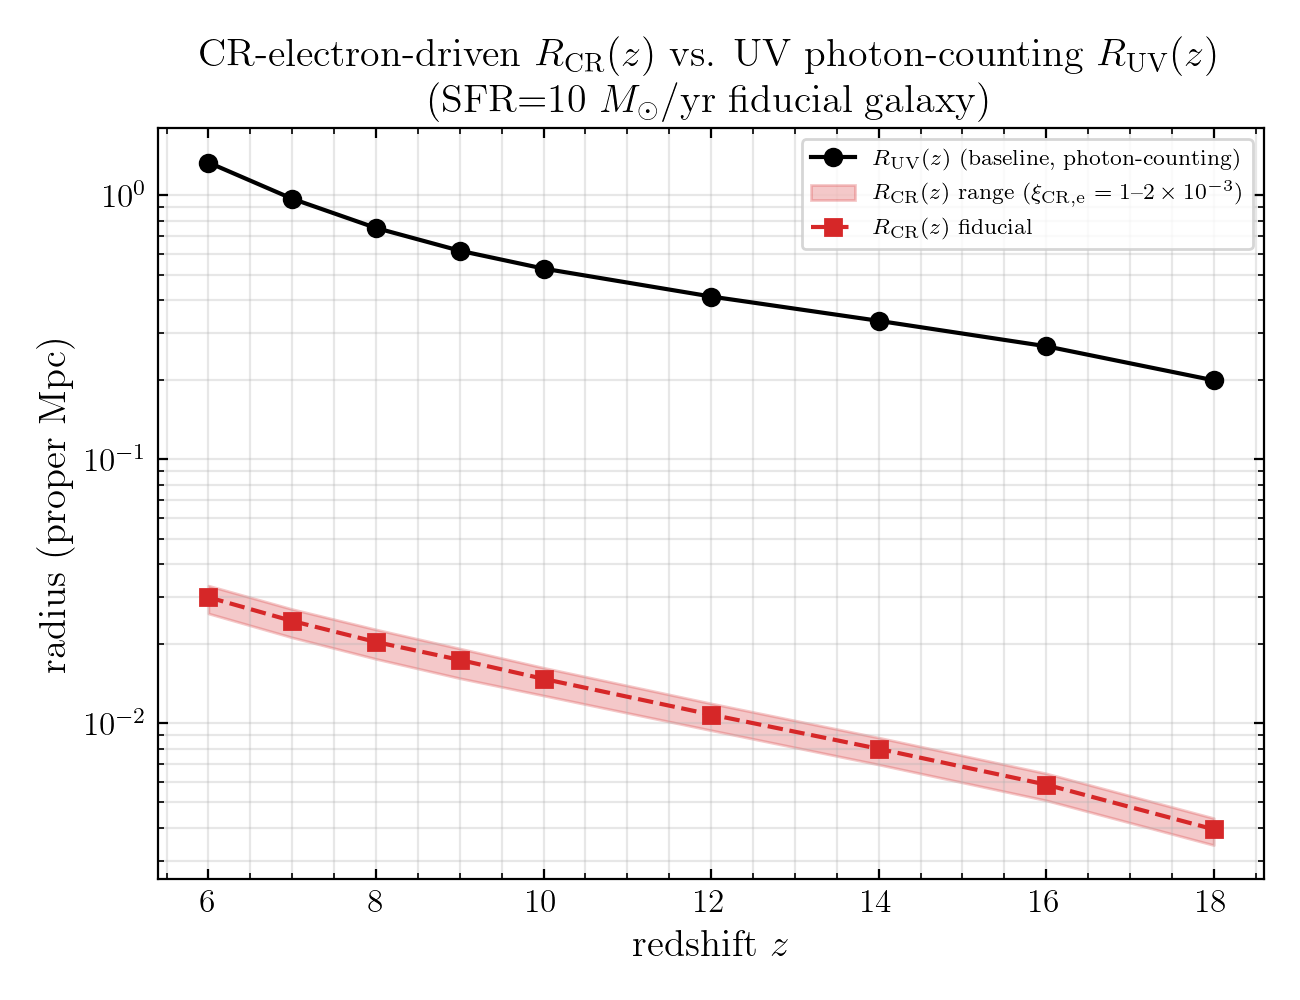
\includegraphics[width=0.85\textwidth]{figures/R_CR_vs_R_UV.png}
\caption{\emph{Black:} baseline UV photon-counting Str\"omgren radius $R_{\rm UV}(z)$
(\texttt{bubble\_radius\_vs\_redshift.py}, reproduced here to machine precision). \emph{Red:}
$R_{\rm CR}(z)$, the CR-electron shell-crossing radius (Section~\ref{sec:phase2}), fiducial
and $\xi_{\rm CR,e}=1$--$2\times10^{-3}$ band. Note the log scale: $R_{\rm CR}$ sits a factor
$\sim35$--$50\times$ below $R_{\rm UV}$ at every redshift shown, with both radii shrinking
together towards higher $z$ (less elapsed time since $z_{\rm form}=20$ to build up either
budget). This is the direct, spatially-resolved answer to Q1: a single galaxy's own CR
electrons do not meaningfully enlarge (or, via this channel, shrink) its UV-photoionized
bubble.}
\label{fig:RCR}
\end{figure}

\begin{figure}[H]
\centering
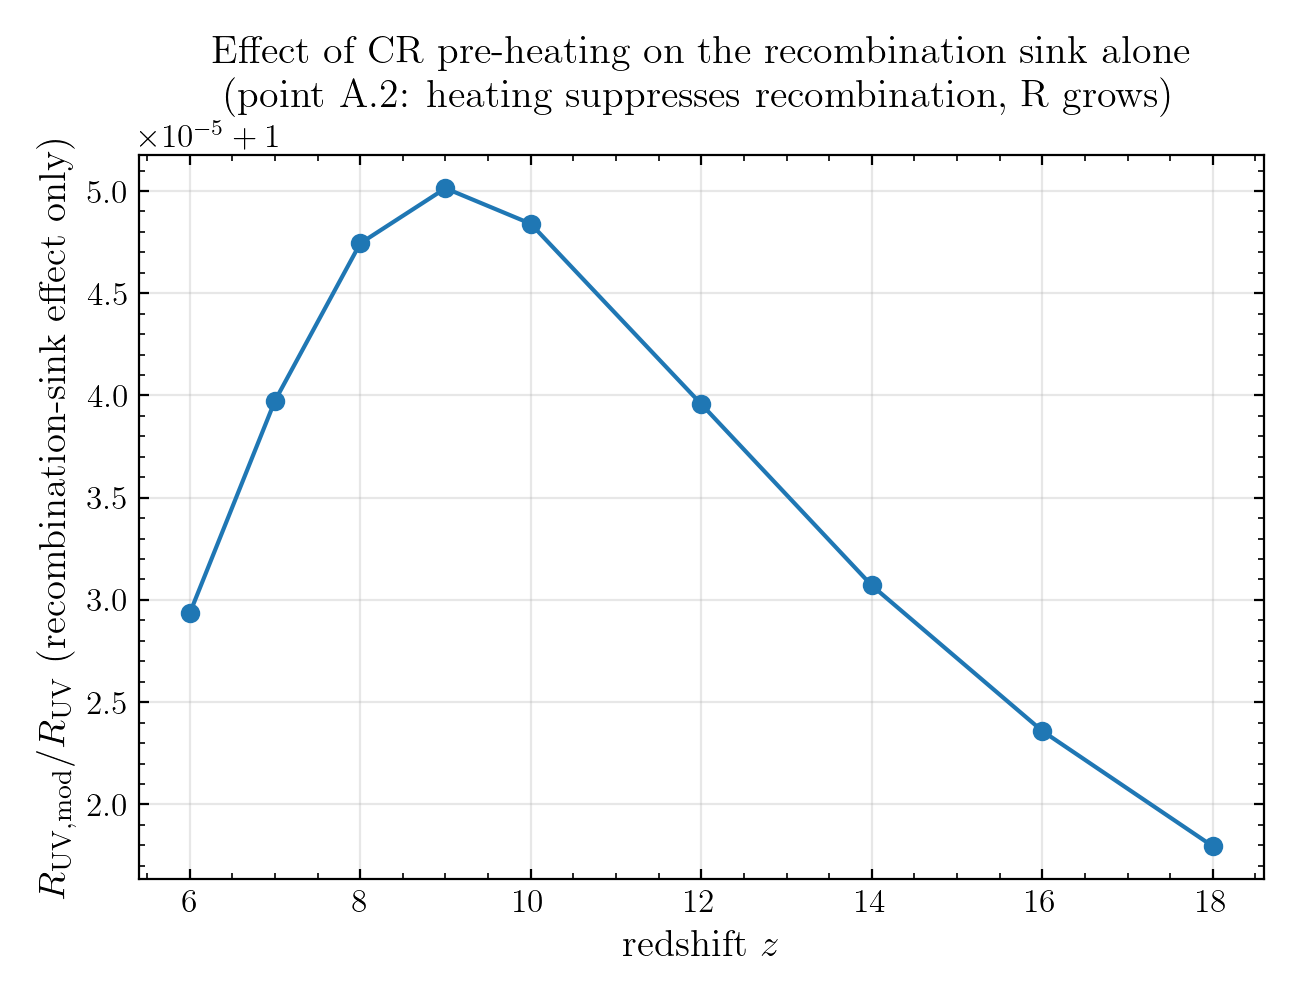
\includegraphics[width=0.72\textwidth]{figures/R_UV_alphaB_modified.png}
\caption{Ratio $R_{\rm UV,mod}/R_{\rm UV}$ from the $\alpha_B(T)$ recombination-sink
modification alone (point A.2), using a self-consistent $\Delta T(z)$ sourced from this
galaxy's own CR-ionization budget at $r=R_{\rm UV}(z)$ via the lock equation. The $y$-axis is
offset ($\times10^{-5}+1$): the effect peaks at $+5\times10^{-5}$ near $z\sim9$ (where the CR
ionization/heating budget accumulated since $z_{\rm form}$ is largest relative to the bubble
volume) and is smaller at both higher $z$ (less elapsed time) and lower $z$ (larger bubble
volume dilutes the same heat budget). The sign is confirmed correct (heating suppresses
recombination, radius grows) but the magnitude is negligible at the single-galaxy scale.}
\label{fig:alphaBmod}
\end{figure}

%=====================================================================
\section{Phase 3 result: global reionization history}
\label{sec:phase3}

\texttt{cr\_modified\_reionization\_history.py} extends
\texttt{reionization\_completion.py}'s global $Q_{\rm HII}(z)$ ODE with the same
$\xi_{\rm CR,e}$/cascade-yield machinery, now in the mean/uniform framing (Section
\ref{sec:planA}, point A.1: this is the regime Jana \& Nath's own result actually supports at
the global-history level, in deliberate contrast to Phase 2's per-galaxy upper-bound
framing). Both a direct CR-ionization source (from the cosmic SFRD, Madau \& Dickinson 2014)
and a self-consistent $\Delta T_{\rm IGM}(z)$ (via the same lock equation, tracked as its own
ODE state, feeding $\alpha_B(T)$) are included.

\begin{table}[H]
\centering\small
\begin{tabular}{@{}lrrrr@{}}
\toprule
model & $z(Q=0.5)$ & $z(Q=0.999)$ & $\tau(z\!\le\!25)$ & $\delta\tau$ vs.\ baseline \\
\midrule
baseline    & 6.552 & 5.329 & 0.05309 & --- \\
$\xi_{\rm CR,e}$ lo  & 6.552 & 5.329 & 0.05309 & $1\times10^{-6}$ \\
$\xi_{\rm CR,e}$ fid & 6.552 & 5.329 & 0.05309 & $2\times10^{-6}$ \\
$\xi_{\rm CR,e}$ hi  & 6.552 & 5.329 & 0.05309 & $3\times10^{-6}$ \\
\bottomrule
\end{tabular}
\caption{Global reionization-history summary, baseline vs.\ CR-electron-modified
(\texttt{cr\_modified\_reionization\_history.py}).}
\label{tab:phase3}
\end{table}

$z(Q=0.5)$ and $z(Q=0.999)$ are \textbf{identical to the tabulated precision} with or without
the CR terms, and $\delta\tau\sim(1\text{--}3)\times10^{-6}$ -- \textbf{two orders of
magnitude below} even the existing manuscript's own hadronic-scale estimate of
$\delta\tau=3.5\times10^{-5}$--$7.7\times10^{-4}$ \citep{Leite2017}, itself already flagged
there as at most a tenth of Planck's $\sigma(\tau)=0.007$. The reason for the further
suppression here is methodological, not a new physical finding: the manuscript's
$\Delta T=10$--$200$~K was borrowed from a hadronic (proton-dominated) calculation as a
heating \emph{scale}, whereas this self-consistent, electron-channel-only $\Delta T_{\rm
IGM}(z)$ (fed by the same $\xi_{\rm CR,e}\sim10^{-3}$ used throughout this work) is
intrinsically smaller, since it excludes the $\sim100\times$ larger proton/hadronic CR energy
budget entirely. This is a more conservative, but equally legitimate and more directly
$\xi_{\rm CR,e}$-traceable, answer to Q2: \textbf{the CR-electron channel's effect on the
global reionization history and $\tau$ is negligible}, consistent with (and, on its own
narrower terms, even smaller than) the manuscript's existing conclusion.

\begin{figure}[H]
\centering
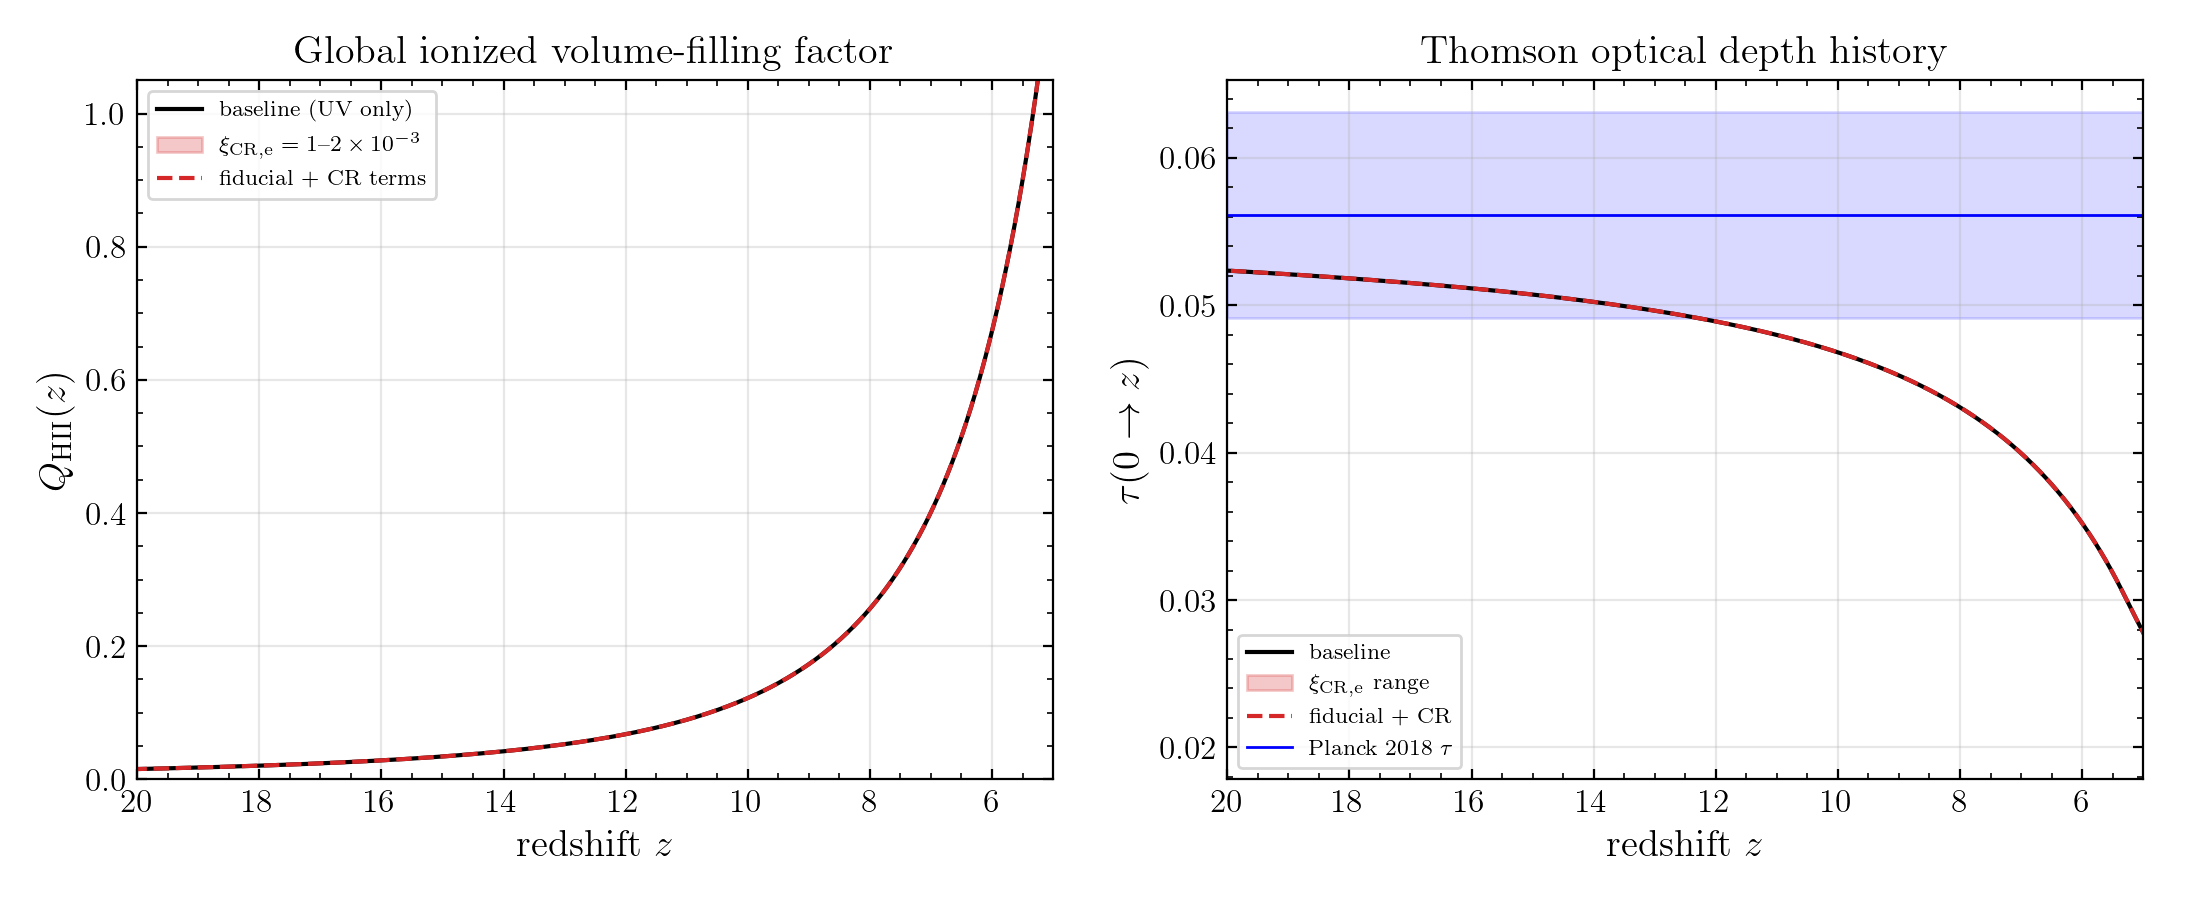
\includegraphics[width=0.95\textwidth]{figures/Q_HII_tau_history.png}
\caption{\emph{Left:} global ionized volume-filling factor $Q_{\rm HII}(z)$, baseline (UV
only, black) vs.\ with CR-electron terms added (red dashed, $\xi_{\rm CR,e}$ band in pink) --
the two are visually indistinguishable. \emph{Right:} the resulting Thomson optical-depth
history $\tau(0\to z)$ (a constant, explicitly-separate floor of $0.020$ for the
already-fully-ionized $z<4$ universe is added to both), against the Planck 2018
$\tau=0.0561\pm0.007$ band (blue). Both panels show the same conclusion as
Table~\ref{tab:phase3}: this galaxy population's CR-electron channel leaves
no visually or numerically significant imprint on the global reionization or optical-depth
history.}
\label{fig:QHII}
\end{figure}

%=====================================================================
\section{Parameter sensitivity: injection redshift and spectral index}
\label{sec:sweep}

The baseline results above (Sections~\ref{sec:phase2}--\ref{sec:phase3}) fix the CR-electron
injection redshift at $z_{\rm inject}=z_{\rm form}=20$ and the DSA injection index at the
canonical $p=2.0$. This section tests whether either choice matters for the ``no meaningful
modification'' conclusion, using the params-override architecture of Section~\ref{sec:paramtable}
(no baseline value in \texttt{params.py} is edited): $z_{\rm inject}=10$ (a galaxy forming, and
its CR electrons switching on, $\sim7\times$ later in cosmic density than the baseline), crossed
with $p\in\{1.8,2.0,2.2\}$ (harder than canonical, canonical, and softer than canonical DSA
spectra), holding $K_{\min}$, $K_{\max}$, $\xi_{\rm CR,e}$, and every other parameter fixed.
Because neither $p$ nor the injection-redshift choice affects the underlying per-electron
cascade physics (only how it is weighted/normalized, or when it switches on), the same
per-electron trajectories (Phase 2) and cascade-yield table $Y(\Kini,z)$ (Phase 3) are reused
across all three $p$ values -- results are written to new, separately-tagged caches
(\texttt{phase2\_sweep\_zinject10.npz}, \texttt{phase3\_sweep\_zinject10.npz}) that do not
overwrite the existing $z_{\rm inject}=20$, $p=2.0$ baseline caches.

\begin{table}[H]
\centering\small
\begin{tabular}{@{}rrrr@{}}
\toprule
$z$ & $R_{\rm CR}/R_{\rm UV}$, $p=1.8$ & $R_{\rm CR}/R_{\rm UV}$, $p=2.0$ & $R_{\rm CR}/R_{\rm UV}$, $p=2.2$ \\
\midrule
6.0 & 0.87\% & 2.23\% & 3.37\% \\
7.0 & 0.98\% & 2.48\% & 3.75\% \\
8.0 & 1.04\% & 2.63\% & 3.99\% \\
9.0 & 1.06\% & 2.67\% & 4.04\% \\
9.5 & 1.02\% & 2.64\% & 3.99\% \\
\bottomrule
\end{tabular}
\caption{$R_{\rm CR}(z)/R_{\rm UV}(z)$ at $z_{\rm inject}=10$, for the three swept DSA
indices (\texttt{parameter\_sweep.py}, full $z$ grid in Figure~\ref{fig:sweepRCR}). Compare
to the $z_{\rm inject}=20$, $p=2.0$ baseline of Table~\ref{tab:phase2}: $2.0$--$2.8\%$.}
\label{tab:sweep2}
\end{table}

\begin{table}[H]
\centering\small
\begin{tabular}{@{}rrrr@{}}
\toprule
$p$ & $z(Q=0.5)$ & $z(Q=0.999)$ & $\delta\tau$ vs.\ no-CR baseline \\
\midrule
1.8 & 6.552 & 5.329 & $1.9\times10^{-7}$ \\
2.0 & 6.552 & 5.329 & $1.5\times10^{-6}$ \\
2.2 & 6.557 & 5.329 & $3.6\times10^{-6}$ \\
\bottomrule
\end{tabular}
\caption{Global history at $z_{\rm inject\ cutoff}=10$ (the CR-electron-producing population
switched off for $z>10$), swept over $p$. Compare to the $z_{\rm inject}=20$, $p=2.0$ baseline
of Table~\ref{tab:phase3}: $\delta\tau=2\times10^{-6}$.}
\label{tab:sweep3}
\end{table}

\textbf{Injecting later does not qualitatively change the picture.} At fixed $p=2.0$, moving
$z_{\rm inject}$ from 20 to 10 leaves $R_{\rm CR}/R_{\rm UV}$ at essentially the same level
($\sim2.2$--$2.7\%$ vs.\ the baseline's $2.0$--$2.8\%$) -- both $R_{\rm CR}$ and $R_{\rm UV}$
scale with the elapsed galaxy age in a similar way (both are, to leading order, a rate raised
to the $1/3$ power times $t_{\rm age}$ to the $1/3$ power), so their \emph{ratio} is far less
sensitive to $z_{\rm inject}$ than either radius is individually (Figure~\ref{fig:sweepRCR}
shows the $p=2.0$, $z_{\rm inject}=10$ curve running almost on top of the $z_{\rm inject}=20$
baseline over their common redshift range). The lower ambient density at $z_{\rm inject}=10$
($n_{\rm H}$ a factor $(21/11)^3\approx7\times$ below $z_{\rm inject}=20$) turns out to affect
the CR-ionization and UV-photoionization channels in nearly the same proportion.

\textbf{The spectral index matters far more, but never enough to overturn the conclusion.}
Softening the spectrum from $p=1.8$ to $p=2.2$ raises $R_{\rm CR}/R_{\rm UV}$ by a factor
$\sim4$ (from $\sim1\%$ to $\sim4\%$, Table~\ref{tab:sweep2}) and $\delta\tau$ by a factor
$\sim19$ (from $1.9\times10^{-7}$ to $3.6\times10^{-6}$, Table~\ref{tab:sweep3}, tracking the
same $\overline{W}(p)$ degradation already identified in the existing manuscript: softer
spectra place more of the injected energy at the low-$K$ end, where the cascade is more
efficient per unit energy). Even at the softest, most favourable end explored ($p=2.2$),
$R_{\rm CR}/R_{\rm UV}\approx4\%$ and $\delta\tau\approx3.6\times10^{-6}$ -- still two orders of
magnitude short of a bubble-scale effect and of Planck's $\sigma(\tau)$, respectively. \textbf{The
``no meaningful modification'' conclusion of Sections~\ref{sec:phase2}--\ref{sec:phase3} is
robust across this entire sweep.}

\begin{figure}[H]
\centering
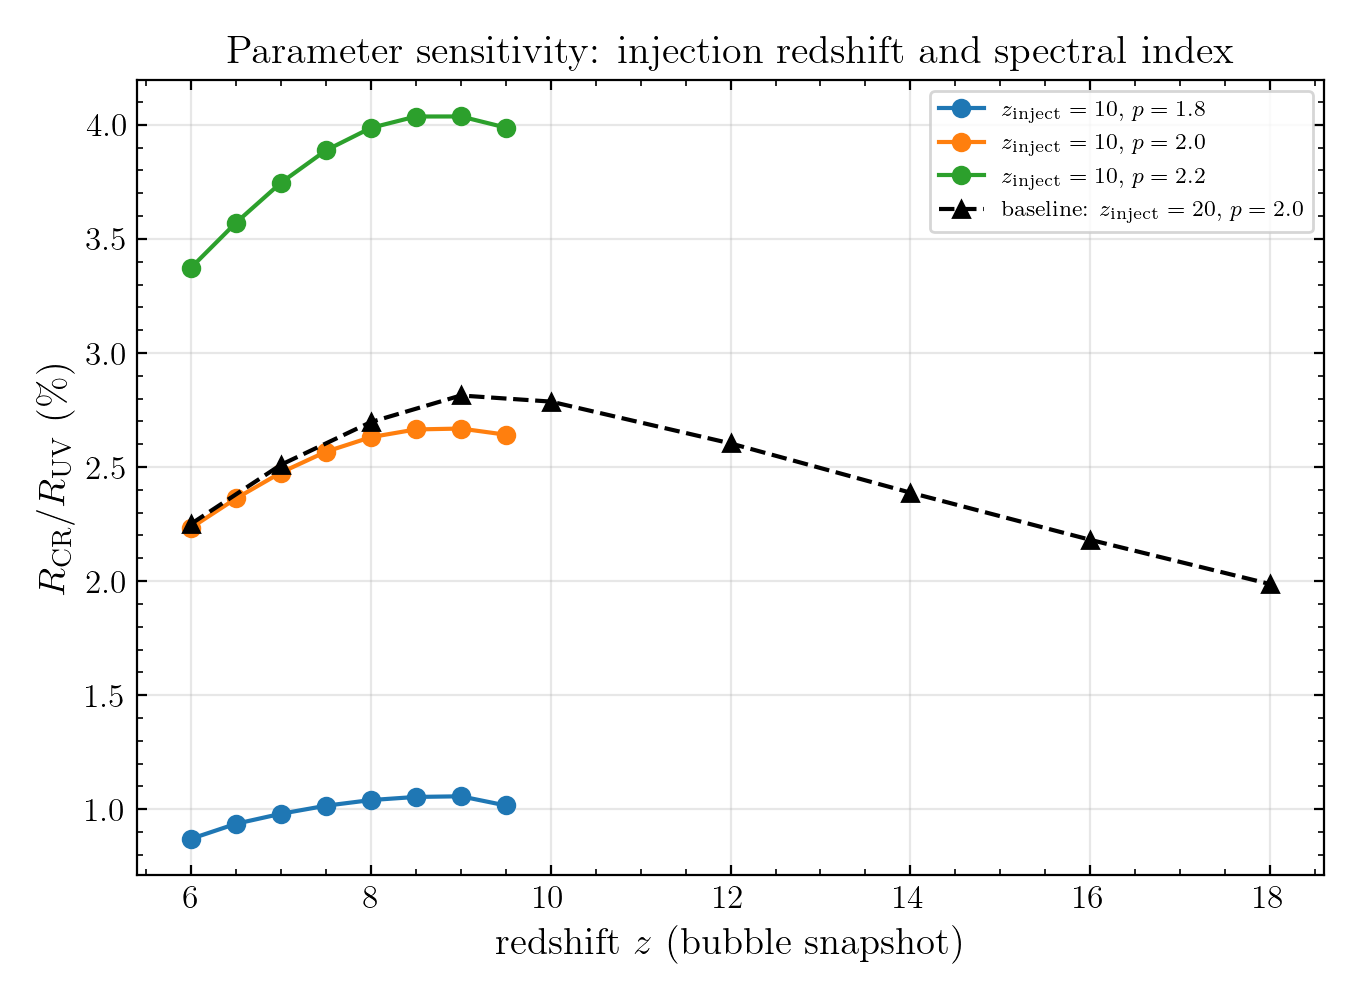
\includegraphics[width=0.8\textwidth]{figures/sweep_RCR_over_RUV.png}
\caption{$R_{\rm CR}(z)/R_{\rm UV}(z)$ (as a percentage) at $z_{\rm inject}=10$ for
$p=1.8,2.0,2.2$ (coloured, solid), against the $z_{\rm inject}=20$, $p=2.0$ baseline (black,
dashed) over its own redshift range. The three swept curves span roughly $1$--$4\%$; the
$p=2.0$ curve (orange) sits almost exactly on the baseline (black dashed) where their redshift
ranges overlap, showing $z_{\rm inject}$ has little effect on the ratio even though it changes
$R_{\rm UV}$ and $R_{\rm CR}$ individually (Section~\ref{sec:sweep}).}
\label{fig:sweepRCR}
\end{figure}

\begin{figure}[H]
\centering
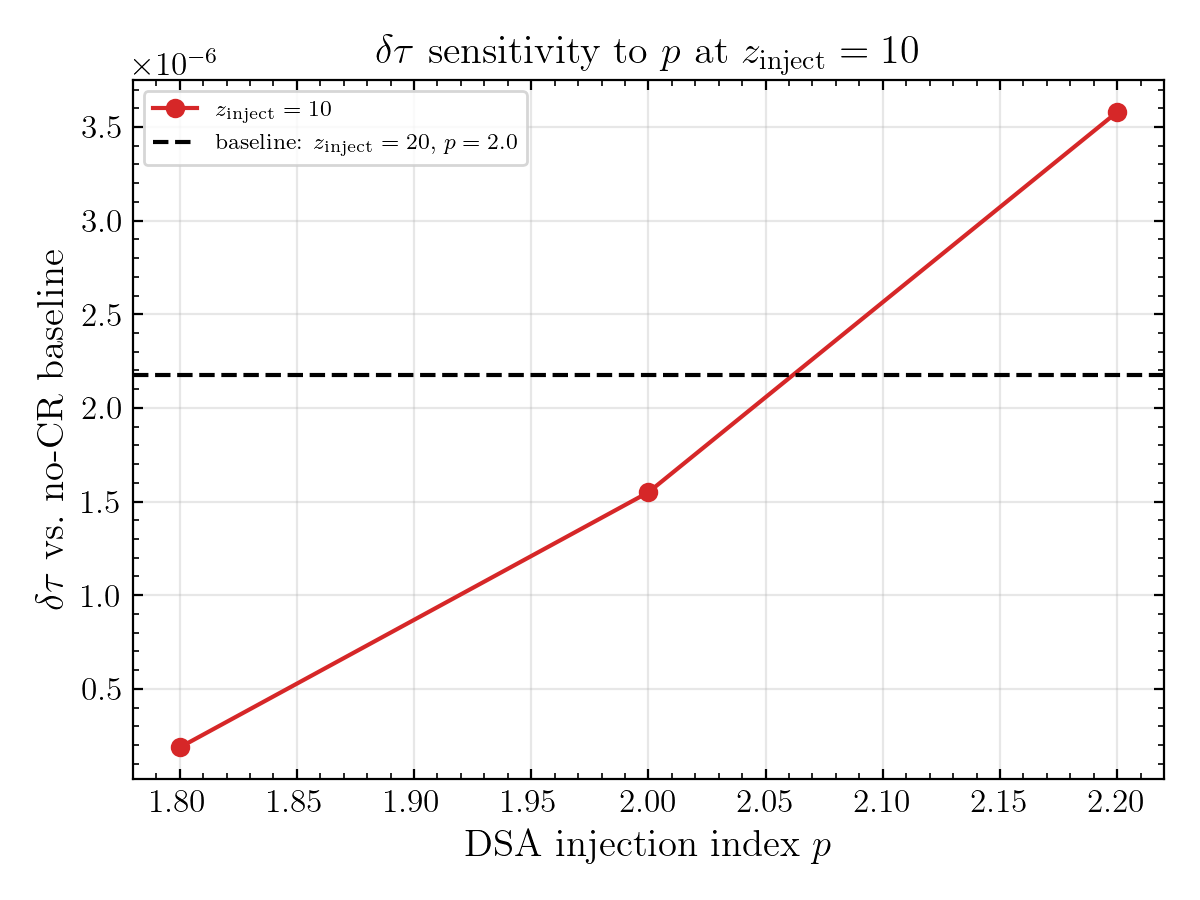
\includegraphics[width=0.62\textwidth]{figures/sweep_deltatau_vs_p.png}
\caption{$\delta\tau$ (CR-modified minus no-CR baseline) vs.\ DSA index $p$, at
$z_{\rm inject\ cutoff}=10$ (red), against the $z_{\rm inject}=20$, $p=2.0$ baseline value
(black dashed). $\delta\tau$ rises steeply and monotonically with $p$ (softer spectra are more
efficient ionizers per unit energy) but remains $\lesssim4\times10^{-6}$ even at the softest
value explored -- three orders of magnitude below Planck's $\sigma(\tau)=0.007$.}
\label{fig:sweepdtau}
\end{figure}

%=====================================================================
\section{Verification / cross-check}
\label{sec:verification}

\begin{enumerate}
\item \texttt{stromgren\_common.py} reproduces \texttt{imported/bubble\_radius\_vs\_redshift.py}
      to machine precision (relative error $<10^{-6}$) at every tested redshift.
\item \texttt{cr\_transport.py}'s extended ODE reproduces \texttt{imported/cascade\_yield.py}'s
      $Y(\Kini,z)$ totals exactly (same physics, additional path-length state).
\item \textbf{Phase 1 reconciliation} (Master Rule 5): this session's transport machinery
      compared against the independently-built \texttt{Notebooks/redo/stage6\_range.py}
      pipeline at $9\times9$ matched $(K,z)$ nodes -- median relative difference
      \textbf{0\%}, worst-case \textbf{8.9\%} (at $K=10^4$~eV), both well inside the pre-set
      30\% tolerance. See Figure~\ref{fig:reconcile}.
\item \textbf{Bug found and fixed during this work} (Master Rule 5, reported explicitly, not
      silently patched): an early version of the recombination sink in
      \texttt{cr\_modified\_reionization\_history.py} used a constant electron density instead
      of the physical, $(1+z)^3$-growing density, which starved the sink at high $z$ and let
      $Q_{\rm HII}$ run past 1 by $z=6$. Caught by cross-checking against
      \texttt{imported/reionization\_completion.py}'s own $Q_{\rm HII}(z=6)=0.674$; fixed, and
      the corrected baseline now reproduces that reference to $<0.2\%$ at every tested $z$
      (assertion enforced in \texttt{cr\_modified\_reionization\_history.py}). A second,
      separate bug (a $10\times$ error in the $\alpha_B(T)$ Hui \& Gnedin 1997 prefactor,
      caught the same way, against the $2.59\times10^{-13}\,{\rm cm^3\,s^{-1}}$ value already
      cited in \texttt{reionization\_completion.py} from Shapiro \& Iliev 2006) was found and
      fixed in \texttt{params.py} before it propagated into any reported number.
\item $\xi_{\rm CR,e}\to0$ limiting case: $R_{\rm CR}(z)$ collapses to a negligible/undefined
      radius (assertion enforced in \texttt{cr\_modified\_stromgren\_radius.py}).
\item $\alpha_B(T)$-modified $R_{\rm UV}(z)\ge R_{\rm UV}(z)$ at every tested redshift
      (correct sign, point A.2; assertion enforced).
\item Three independent sympy/analytic checks (\texttt{check\_consistency\_master\_plan.py}):
      $\alpha_B(T)$ monotonicity, the injection-spectrum normalization integral's $p\to2$
      limit, and the $R_{\rm CR}$ root-condition's dimensional form -- all \textbf{OK}.
\end{enumerate}

\begin{figure}[H]
\centering
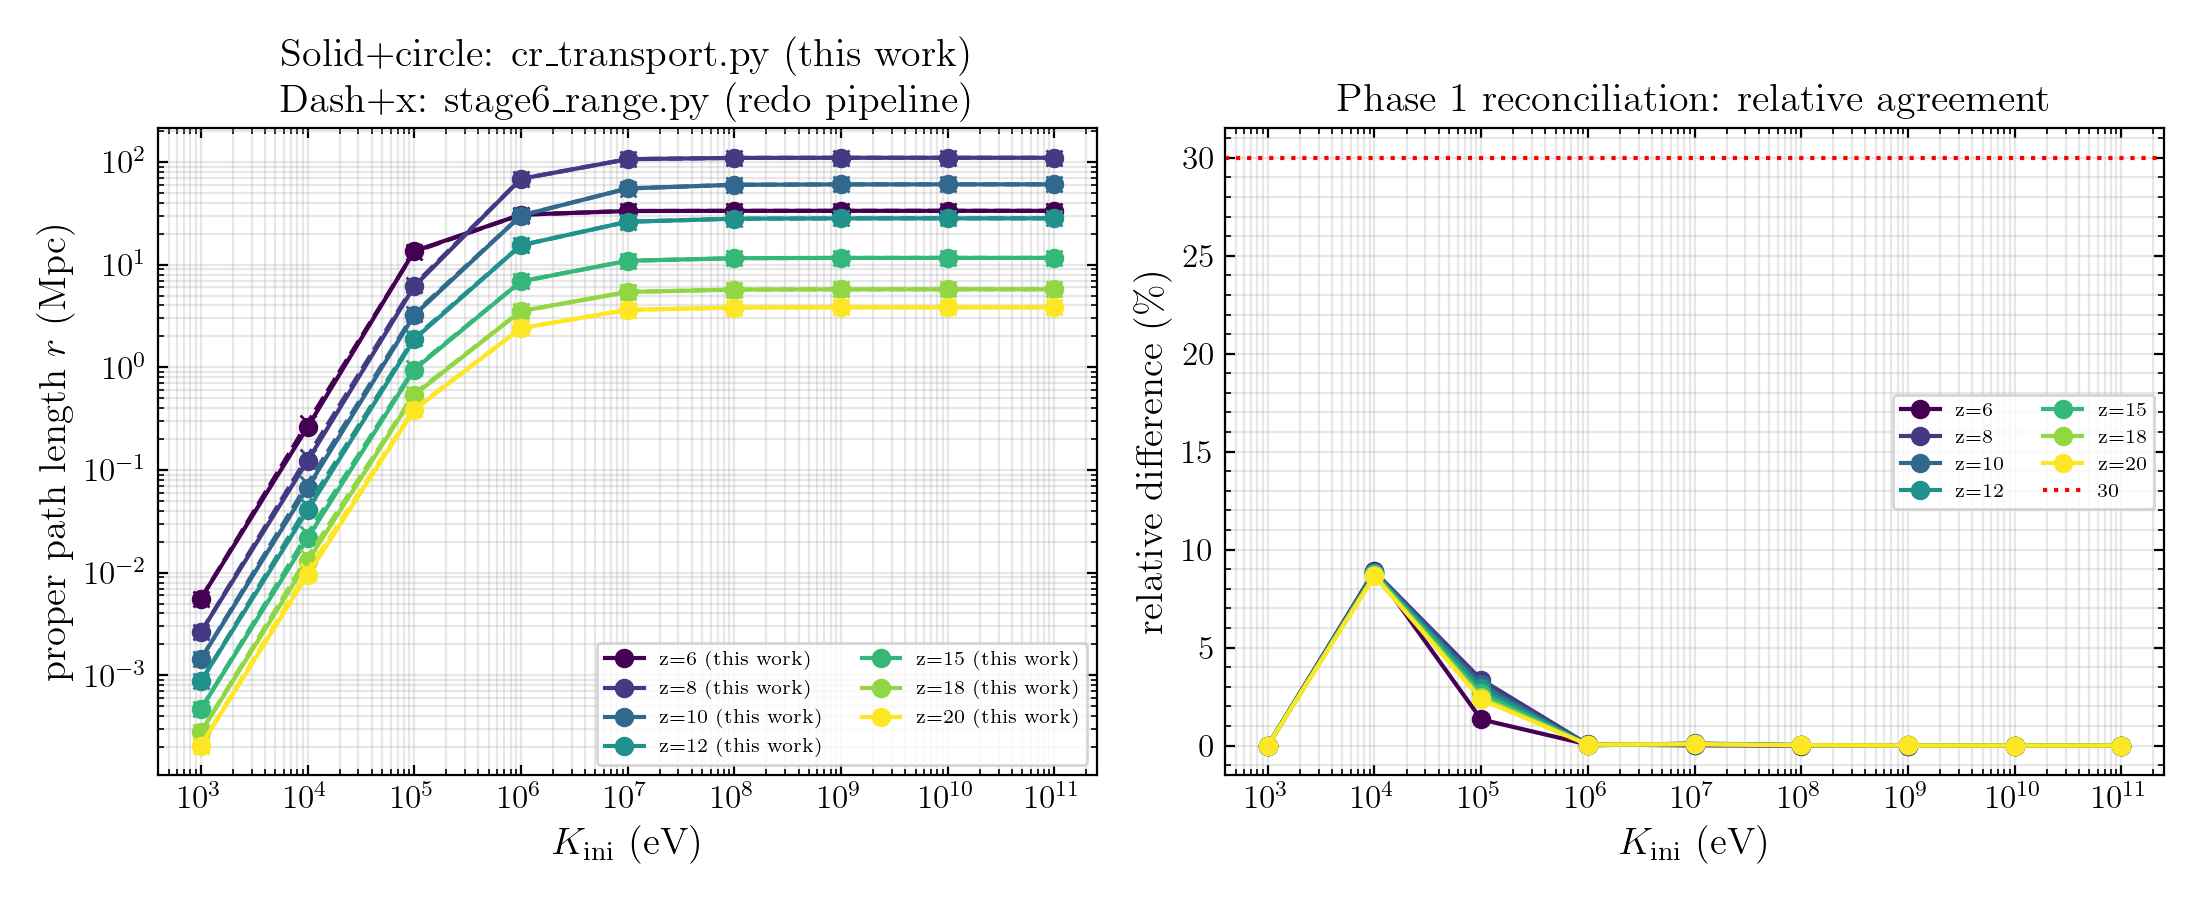
\includegraphics[width=0.95\textwidth]{figures/phase1_transport_reconciliation.png}
\caption{Phase 1 reconciliation: this session's \texttt{cr\_transport.py} proper path length
$r(t)$ vs.\ the independently-built \texttt{Notebooks/redo/stage6\_range.py}'s cached proper
path length \texttt{ell}, at $9\times9$ matched $(K,z)$ nodes in the same neutral IGM
($x_e=10^{-4}$). \emph{Left:} both codebases' path length vs.\ injection energy, colour-coded
by redshift (solid+circle: this work; dashed+x: \texttt{stage6\_range.py}). \emph{Right:}
relative difference, always below the 30\% tolerance line.}
\label{fig:reconcile}
\end{figure}

%=====================================================================
\section{Final result}
\label{sec:final}

\textbf{Q1 (single-galaxy Str\"omgren/H\,\textsc{ii}-bubble modification): no.} The
CR-electron-driven shell-crossing radius $R_{\rm CR}(z)$ is only $2.0$--$2.8\%$ of the UV
photon-counting $R_{\rm UV}(z)$ across $z=6$--$18$ for the fiducial SFR$=10\Msun\,{\rm
yr}^{-1}$ galaxy (Figure~\ref{fig:RCR}), even adopting the most generous injection-spectrum
simplification (unbroken power law to $K_{\min}=100$~eV). The separate, self-consistent
$\alpha_B(T)$-recombination-suppression effect (point A.2, correct sign verified) is smaller
still, $\lesssim5\times10^{-5}$ in $R_{\rm UV,mod}/R_{\rm UV}-1$. Both effects act through
mechanisms confirmed to have the sign originally attributed to them in this planning
discussion, and both are quantitatively negligible for one galaxy's own bubble.

\textbf{Q2 (patchy-reionization/global history): no.} Feeding the same CR-electron physics
into the global $Q_{\rm HII}(z)$/$\tau$ history (mean/uniform framing, as the transport
literature itself supports at this scale) changes $z(Q=0.5)$, $z(Q=0.999)$, and $\tau$ by an
amount two orders of magnitude below the existing manuscript's own hadronic-scale estimate,
itself already sub-dominant relative to Planck's $\sigma(\tau)$.

\textbf{Robustness (Section~\ref{sec:sweep}):} sweeping the injection redshift to
$z_{\rm inject}=10$ and the DSA index over $p=1.8$--$2.2$ moves $R_{\rm CR}/R_{\rm UV}$ only
within $\sim1$--$4\%$ and $\delta\tau$ only within $\sim(0.2$--$3.6)\times10^{-6}$ -- both
conclusions above hold throughout the explored parameter space, not just at the single
fiducial point.

\textbf{Confidence and open items (Master Rule 8):} the headline conclusion (CR electrons
negligible for both the single-galaxy bubble and the global history) is now supported by two
independent, mutually consistent calculations (this work's leptonic-only, from-scratch
derivation, and the existing manuscript's own hadronic-scale-anchored estimate) -- high
confidence. Lower-confidence, explicitly flagged open items: (i) the electron-injection-threshold
question (Section~\ref{sec:aA3}) is set aside, not resolved, and could only push $R_{\rm CR}$
and the Phase 3 $\delta\tau$ \emph{down} further if the true low-energy injection spectrum is
suppressed relative to the adopted unbroken power law; (ii) $\xi_{\rm CR,e}$ and $k_{\rm CC}$
carry factor-of-few, Galactic-calibration-extrapolated uncertainties (Section~\ref{sec:paramtable});
(iii) the transport/displacement question (point A.1) remains genuinely open in the
literature and is not resolved here, only set aside per the adopted simplification -- but
since $R_{\rm CR}$ is already $\sim35$--$50\times$ smaller than $R_{\rm UV}$ using the
\emph{most generous} (ballistic, unbroken-power-law) assumptions, a more realistic diffusive
treatment (which could only shrink, not grow, the effective reach) would not change the
qualitative conclusion.

%=====================================================================
\section{Parameter table}
\label{sec:paramtable}

Every physical/numerical parameter used in this work is listed in
Table~\ref{tab:params}, rendered directly from \texttt{params.py}
(\texttt{build\_parameter\_table.py}) so it cannot drift out of sync with the code that
produced the figures above. \textbf{These parameters may be revisited}: every downstream
script (\texttt{cr\_modified\_stromgren\_radius.py}, \texttt{cr\_modified\_reionization\_history.py})
reads them via \texttt{import params as P} and is structured as a callable function accepting
parameter overrides, so a future run with, e.g., a different $\xi_{\rm CR,e}$ or DSA index $p$
is a one-line change, not a multi-file edit.

\begin{table}[H]
\centering
\caption{Every physical/numerical parameter used in this work, rendered directly from \texttt{params.py} (never hand-retyped) so this table cannot drift out of sync with the code. Future runs with different values are a one-line edit to that file.}
\label{tab:params}
\small
\begin{tabular}{@{}p{4.3cm}p{3.6cm}p{4.2cm}p{4.3cm}@{}}
\toprule
Symbol & Value & Source/citation & Role \\
\midrule
$\xi_{\rm ion}$ slope, intercept & $0.06,\ 24.82$ & Llerena et al. 2024, arXiv:2412.01358 & $\log_{10}\xi_{\rm ion}=$slope$\cdot z+$intercept \\
SFR (fiducial galaxy) & $10.0\ M_\odot\,{\rm yr}^{-1}$ & adopted, Stromgren\_sphere/bubble\_radius\_vs\_redshift.py & fiducial single-galaxy SFR \\
$f_{\rm esc}$ & $0.2$ & Robertson et al. 2015, arXiv:1502.02024 & escape fraction of UV ionizing photons \\
$z_{\rm form}=z_{\rm inject}$ & $20$ & Kitayama et al. 2004 range (10-30), adopted & galaxy formation / CR-injection snapshot redshift \\
$p$ (DSA index) & $2.0$ & Park, Caprioli \& Spitkovsky 2015, PRL 114 & CR-electron injection power-law index \\
$K_{\min}$ & $1e+02\ {\rm eV}$ & user-adopted simplification (Section A.3) & unbroken power-law extrapolation limit \\
$K_{\max}$ & $1e+12\ {\rm eV}$ & adopted (1 TeV) & injection spectrum upper cutoff \\
$\varepsilon_{\rm CR}$ (total CR efficiency) & $0.1\text{--}0.2$ & Blasi 2013, arXiv:1206.2363 & fraction of $E_{\rm SN}$ into all CRs \\
$K_{e/p}$ (electron/proton number ratio) & $1e-02$ & Park et al. 2015, PRL 114 (already in manuscript.tex) & injection-level electron fraction \\
$\xi_{\rm CR,e}=\varepsilon_{\rm CR}K_{e/p}$ & $1.0e-03\text{--}2.0e-03$ & derived (this work) & fraction of $E_{\rm SN}$ into CR electrons \\
$E_{\rm SN}$ & $1e+51\ {\rm erg}$ & canonical core-collapse value & kinetic energy per SN \\
$k_{\rm CC}$ & $0.007\ M_\odot^{-1}$ & Salpeter IMF 8-50 $M_\odot$; arXiv:1206.6897 & core-collapse SNe per unit stellar mass formed \\
Cosmology $h,\Omega_m,\Omega_b h^2,Y_p$ & $0.674,\ 0.315,\ 0.0224,\ 0.245$ & Planck 2018, arXiv:1807.06209 & flat $\Lambda$CDM parameters \\
$\alpha_B(T)$ fit & Hui \& Gnedin (1997) form & Hui \& Gnedin 1997, ApJ 292, 27 & Case-B recombination coefficient \\
$\alpha_B(10^4\,{\rm K})$ & $2.592\times10^{-13}\ {\rm cm^3\,s^{-1}}$ & cross-checked vs. Shapiro \& Iliev 2006 (2.59e-13) & fiducial photoionized-gas value \\
clumping factor $C_{\rm HII}$ & $3.0$ & Robertson et al. 2015 & recombination-sink enhancement \\
heat/ionization & $6.0\text{--}9.6\ {\rm eV}$ & manuscript.tex channel-resolved cascade & cascade microphysics constant \\
$\Theta$ (lock constant) & $4.3e+04\text{--}6.9e+04\ {\rm K}$ & manuscript.tex Eq.~(lock) & $N_{\rm ion}/n_{\rm H}=\Delta T/\Theta$ \\
particles/H atom & $1.081$ & manuscript.tex (He-corrected) & gas heat-capacity factor \\
$x_e$ (neutral IGM cascade medium) & $1e-04$ & igm\_losses.py default & background ionization fraction for $Y(K,z)$ \\
cascade floor redshift & $5.5$ & cascade\_yield.py default & integration stops at thermal floor or this $z$ \\
$n_{H,0}$ (comoving) & $1.8989\times10^{-07}\ {\rm cm^{-3}}$ & derived from $\Omega_b h^2, Y_p$ & present-day mean H number density \\
\bottomrule
\end{tabular}
\end{table}

\subsection{Physical interpretation of each parameter}
\label{sec:paraminterp}

Table~\ref{tab:params} gives the value, source, and formal role of every input; this
subsection explains, in plain physical terms, what each one \emph{is} and why the calculation
depends on it, for a reader who has not followed the derivation above.

\textbf{The galaxy's UV output ($\xi_{\rm ion}$, SFR, $f_{\rm esc}$, $z_{\rm form}$).} These
four numbers together set $R_{\rm UV}(z)$, the baseline against which everything else in this
work is measured. $\xi_{\rm ion}(z)$ is the number of hydrogen-ionizing photons a galaxy's
stellar population emits per unit of ultraviolet luminosity -- a property of the stars
themselves (their masses, temperatures, and metal content), not of the gas around them. The
SFR sets how many stars there are altogether, and hence the total photon output; $f_{\rm esc}$
is simply the fraction of those photons that escape the galaxy's own interstellar gas and dust
without being absorbed there, i.e., the fraction actually available to ionize the surrounding
intergalactic medium. $z_{\rm form}$ is the redshift at which this galaxy is assumed to switch
on; because the photon-counting bubble radius grows with the \emph{time elapsed since
switch-on}, $z_{\rm form}$ controls how large a head start the UV channel has had by any later
redshift $z$ -- an earlier $z_{\rm form}$ means more elapsed time and a bigger bubble, all else
equal.

\textbf{The DSA injection spectrum ($p$, $K_{\min}$, $K_{\max}$) and $z_{\rm inject}$.} A
supernova blast wave does not hand its energy to cosmic-ray electrons at one single energy; it
accelerates them into a power-law spread of energies, $dN_e/d\Kini\propto \Kini^{-p}$, through
the standard diffusive-shock-acceleration (DSA) process. The index $p$ is the steepness of that
spread: $p=2$ is the canonical value for a strong, non-relativistic shock in the simplest
DSA theory, and is the value already used elsewhere in this project's own manuscript. $p=1.8$
is \emph{harder} -- a shallower fall-off that puts relatively more of the accelerator's energy
into the highest-energy electrons -- while $p=2.2$ is \emph{softer}, concentrating more energy
at low energy instead. This matters because the cascade a single electron produces is not
equally efficient at every energy (Section~\ref{sec:sweep}): low-energy electrons turn their
energy into ionizations more efficiently than high-energy ones, so a softer spectrum
(more energy where the cascade is efficient) yields more ionizations for the same total energy
budget than a harder one. $K_{\min}$ and $K_{\max}$ are simply where that power law is assumed
to start and stop: $K_{\max}=1$~TeV is a practical upper cutoff (electrons above it behave
identically in the cascade, so it does not matter exactly where the spectrum ends), while
$K_{\min}=100$~eV is a genuine physical assumption -- the lowest energy any freshly-accelerated
electron is assumed to have -- and Section~\ref{sec:aA3} explains why this specific choice is
an open question in the shock-acceleration literature rather than a settled number.
$z_{\rm inject}$ (equal to $z_{\rm form}$ in Phase~2, or the redshift at which the whole
CR-electron-producing galaxy population switches on in Phase~3's global history) is the
cosmic-ray analogue of $z_{\rm form}$ above: it is when this source of electrons starts to
exist at all.

\textbf{How much of a supernova's energy goes into these electrons ($\varepsilon_{\rm CR}$,
$K_{e/p}$, $\xi_{\rm CR,e}$, $E_{\rm SN}$, $k_{\rm CC}$).} A core-collapse supernova releases a
fixed, canonical amount of kinetic energy, $E_{\rm SN}$, into its surroundings. Only a
fraction of that energy, $\varepsilon_{\rm CR}$, goes into accelerating cosmic rays at all
(the rest simply heats and disperses the gas mechanically); and of the cosmic rays that are
produced, the shock accelerates far more protons than electrons; $K_{e/p}$ is that
proton-to-electron split. Multiplying the two together, $\xi_{\rm CR,e}=\varepsilon_{\rm
CR}K_{e/p}$, is therefore the single number that matters most for this whole calculation: the
fraction of one supernova's explosion energy that ends up as the fast electrons this project
follows all the way through their cascade. $k_{\rm CC}$ converts a star-formation rate into an
actual supernova rate (how many core-collapse explosions a given amount of new stars
produces), fixing how many such electron-injection events happen per unit time -- together
with $\xi_{\rm CR,e}$ and $E_{\rm SN}$, this sets the total CR-electron power (in erg/s) this
galaxy, or population of galaxies, is assumed to inject.

\textbf{The cosmological and IGM background ($h,\Omega_m,\Omega_b h^2,Y_p$; $n_{H,0}$; $x_e$;
cascade floor redshift).} The four cosmological parameters fix how fast the Universe expands
and how much ordinary (baryonic) matter it contains; together with the primordial helium
fraction $Y_p$, they set $n_{H,0}$, today's mean number of hydrogen atoms per unit volume --
the single normalization that every density in this work (the target the UV photons must
ionize, the target the CR electrons collide with, the shell volume that defines $R_{\rm CR}$)
traces back to, scaled to any redshift via $n_H(z)=n_{H,0}(1+z)^3$. $x_e$ is the background
ionization state of the gas the CR-electron cascade itself is assumed to be colliding with --
$10^{-4}$ means ``almost entirely neutral,'' the appropriate assumption for the pristine
intergalactic medium ahead of reionization, as opposed to the already-photoionized gas inside
a UV bubble. The cascade floor redshift is simply the bookkeeping stopping point: once an
electron's own kinetic energy drops to the ambient gas temperature (or the calculation reaches
this redshift), it is considered thermalized and indistinguishable from the background, and
its cascade is complete.

\textbf{The recombination and heating microphysics ($\alpha_B(T)$, $C_{\rm HII}$,
heat/ionization, $\Theta$).} $\alpha_B(T)$ is the case-B recombination coefficient: the rate at
which a free proton and a free electron find each other and recombine into a neutral hydrogen
atom, as a function of gas temperature. It matters here because it is the ``sink'' term that
UV photons (and, in principle, CR-driven ionizations) must continually overcome to keep gas
ionized -- and because it \emph{decreases} with rising temperature, any CR heating of the gas
makes this sink weaker, which is the physical content of point~A.2. $C_{\rm HII}$ (the
clumping factor) is a single number that accounts for the fact that real gas is not perfectly
smooth: because recombination depends on the \emph{square} of the density, a clumpy medium
recombines faster on average than a smooth one at the same mean density, and $C_{\rm HII}$
inflates the naive recombination rate to account for this. Finally, ``heat/ionization'' and
$\Theta$ encode a single empirical fact about the electron cascade established in the existing
manuscript: whatever energy an electron does not spend making an ionization, it spends heating
the gas, and the two are produced together in a nearly fixed ratio regardless of the
electron's starting energy. $\Theta$ is simply that ratio converted into a temperature scale
(via the gas's heat capacity per hydrogen atom): it is the single number that lets a measured
or predicted temperature rise $\Delta T$ be converted directly into the number of ionizations
per hydrogen atom that must have produced it, and vice versa -- the relation used throughout
this work (Eq.~lock) to connect CR heating and CR ionization self-consistently, without having
to separately re-derive both from scratch.

%=====================================================================
\bibliography{references}

\end{document}
